\documentclass[aspectratio=169, 12pt]{beamer}

\usetheme{Madrid}
\usecolortheme{seahorse}

% --- Dark theme ---
\setbeamercolor{background canvas}{bg=black!90}
\setbeamercolor{normal text}{fg=white}
\setbeamercolor{frametitle}{fg=white, bg=black!70}
\setbeamercolor{title}{fg=white}
\setbeamercolor{subtitle}{fg=white!80}
\setbeamercolor{author}{fg=white!80}
\setbeamercolor{date}{fg=white!70}
\setbeamercolor{institute}{fg=white!70}
\setbeamercolor{item}{fg=cyan!70}
\setbeamercolor{block title}{fg=white, bg=cyan!40!black}
\setbeamercolor{block body}{bg=black!60}
\setbeamercolor{structure}{fg=cyan!70}
\setbeamercolor{alerted text}{fg=yellow!80}

\usepackage{graphicx}
\usepackage{amsmath}
\usepackage{booktabs}
\usepackage{hyperref}
\usepackage{xcolor}
\usepackage{tikz}

% highlight box
\newcommand{\hlbox}[2]{%
  \colorbox{#1}{\strut\color{white}\bfseries\,#2\,}%
}

\title{Real-Time Visualization of Digital Modulation\\and Channel Impairments Using a Single PlutoSDR}
\author{Howard Wang}
\institute{ENGR 78 -- Final Project}
\date{Spring 2026}

\begin{document}

% ==================================================================
% SLIDE 1 -- Title
% ==================================================================
\begin{frame}[plain]
\titlepage
\end{frame}

% ==================================================================
% SLIDE 2 -- The Problem
% ==================================================================
\begin{frame}{The Problem}
\begin{center}
\Large\color{yellow!80}
``I can solve the BER equation, but I have no idea\\
what a noisy constellation \emph{looks} like.''
\end{center}
\vspace{0.8cm}
\begin{itemize}
    \item Traditional courses: modulation = equations + static textbook plots
    \item Students memorize $Q\!\bigl(\sqrt{2E_b/N_0}\bigr)$ but never \textbf{watch} a signal degrade
    \item Gap between theory and physical intuition
\end{itemize}
\vfill
\begin{block}{}
\centering\textbf{What if you could \emph{see} every impairment happen in real time, on real hardware?}
\end{block}
\end{frame}

% ==================================================================
% SLIDE 3 -- What We Built
% ==================================================================
\begin{frame}{What We Built}
\begin{columns}[c]
\begin{column}{0.55\textwidth}
A \alert{real-time, interactive} digital-communications workbench:
\vspace{0.4cm}
\begin{enumerate}
    \item Generate \& transmit a digital signal through an \hlbox{red!60}{ADALM-PLUTO SDR}
    \item Receive it back via loopback (or software simulation)
    \item Inject impairments with sliders --- \textbf{instantly} see the effect
    \item Five live panels: spectrum, constellation, eye diagram, metrics, \textbf{throughput}
    \item Automated \hlbox{blue!50}{BER sweep mode} for quantitative analysis
\end{enumerate}
\end{column}
\begin{column}{0.42\textwidth}
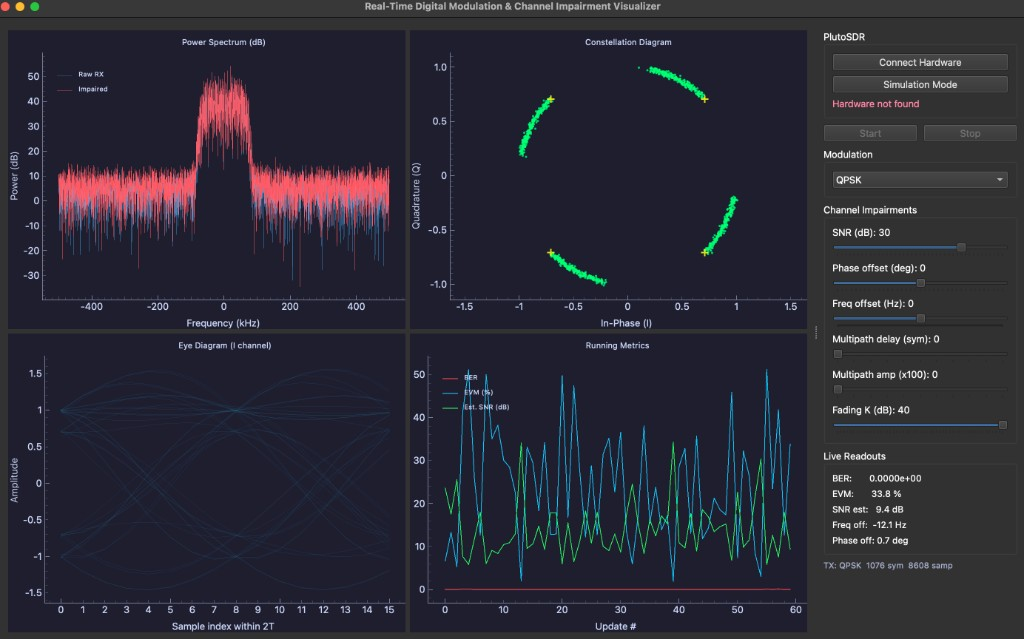
\includegraphics[width=\textwidth]{figures/gui_live.png}
\end{column}
\end{columns}
\end{frame}

% ==================================================================
% SLIDE 4 -- System Architecture
% ==================================================================
\begin{frame}{System Architecture}
\begin{center}
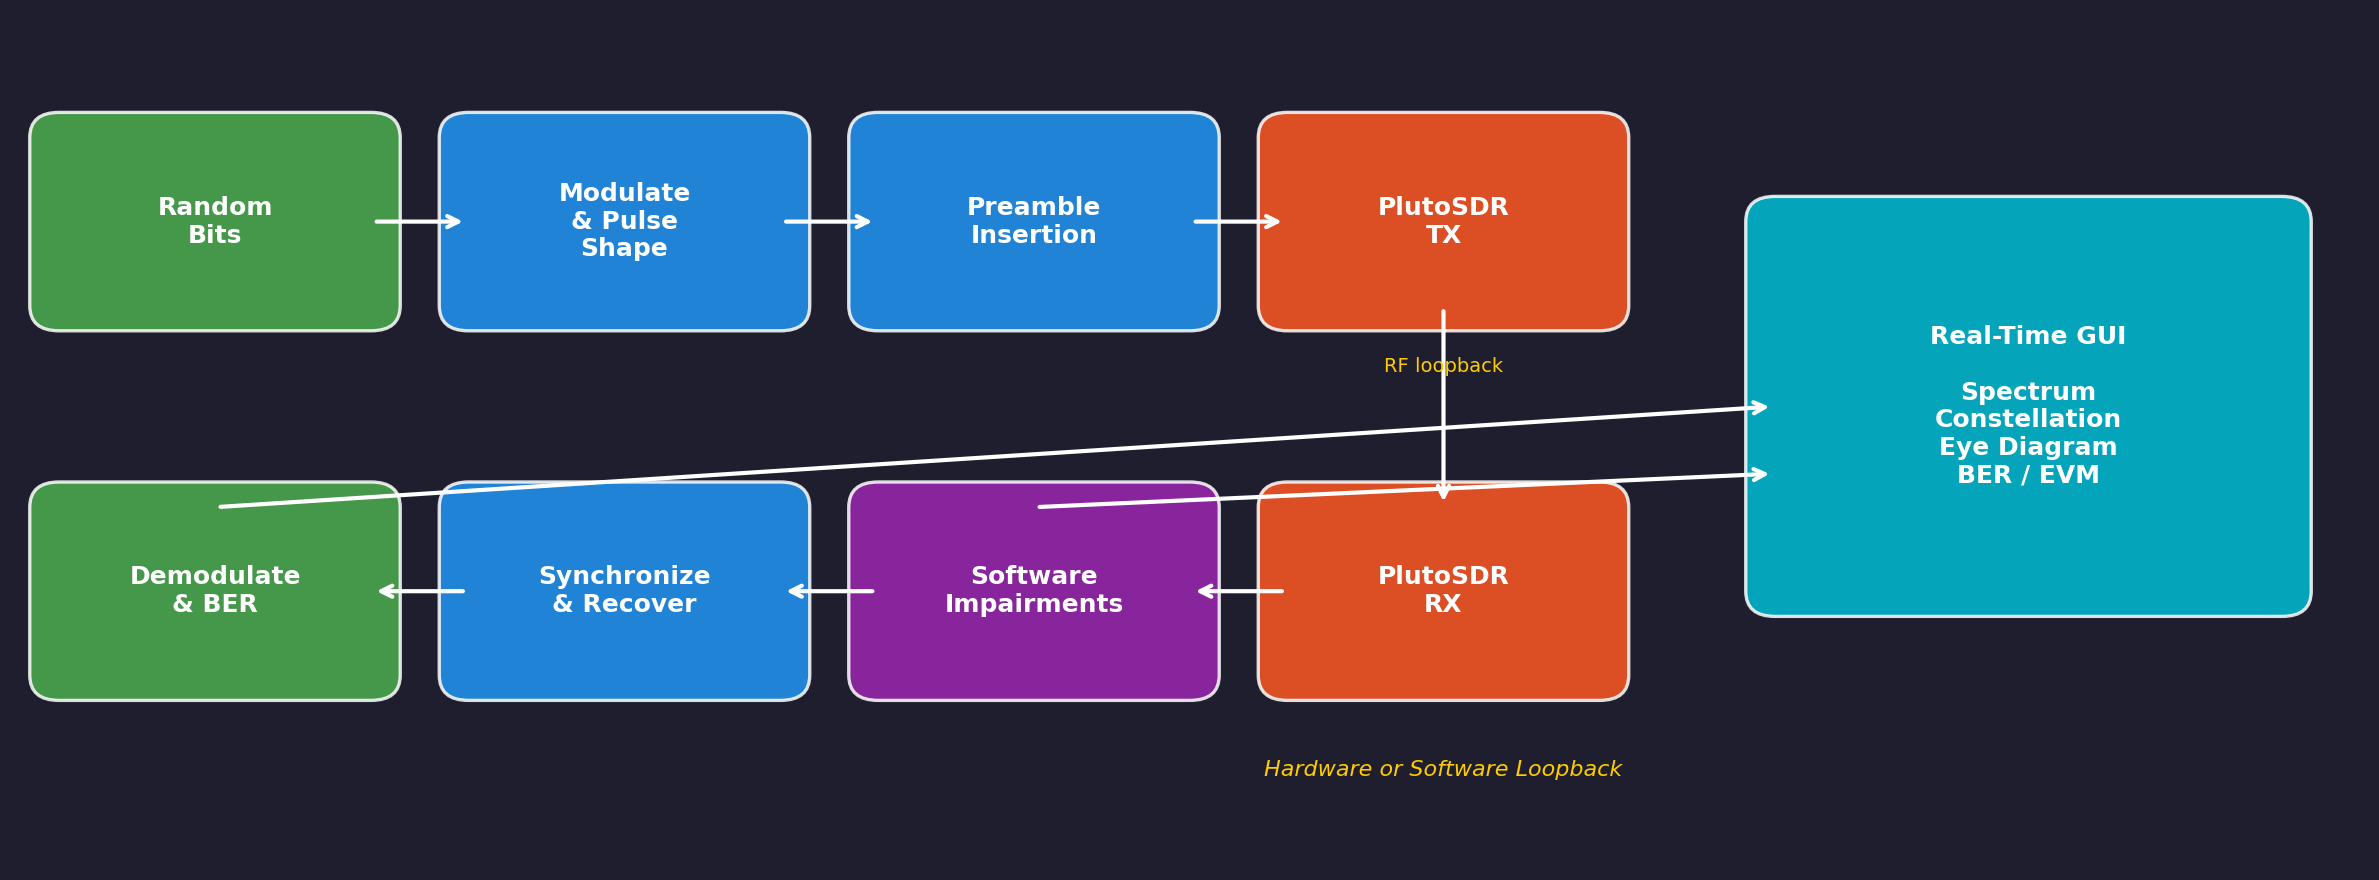
\includegraphics[width=0.88\textwidth]{figures/block_diagram_v2.png}
\end{center}
\vspace{-0.1cm}
\begin{columns}[T]
\begin{column}{0.48\textwidth}
\begin{itemize}
    \item \hlbox{red!60}{PlutoSDR} TX $\to$ 30\,dB attenuator $\to$ RX
    \item Falls back to \hlbox{blue!50}{software loopback} if no hardware
\end{itemize}
\end{column}
\begin{column}{0.48\textwidth}
\begin{itemize}
    \item Impairments injected \textbf{post-RX} -- no TX rebuild needed
    \item GUI polls worker at 20 FPS -- DSP decoupled from rendering
\end{itemize}
\end{column}
\end{columns}
\end{frame}

% ==================================================================
% SLIDE 5 -- Modulation Schemes
% ==================================================================
\begin{frame}{Four Modulation Schemes}
\begin{center}
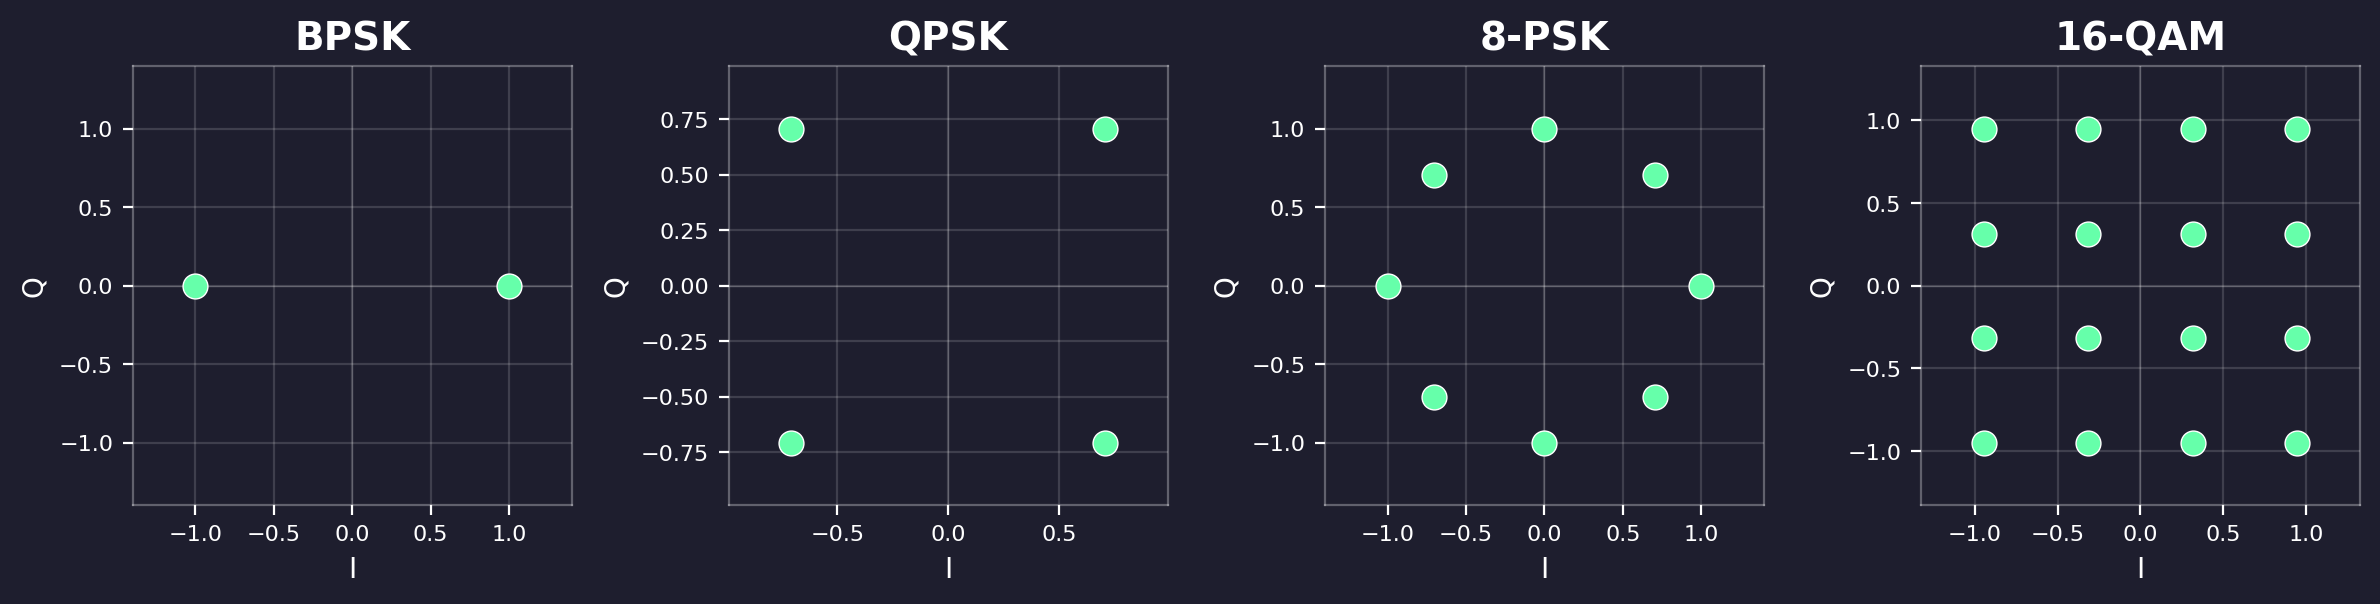
\includegraphics[width=0.92\textwidth]{figures/constellations.png}
\end{center}
\vspace{-0.1cm}
\begin{columns}[T]
\begin{column}{0.48\textwidth}
\begin{itemize}
    \item Gray-coded constellations
    \item Root-raised-cosine pulse shaping ($\alpha\!=\!0.35$, 8 samp/sym)
\end{itemize}
\end{column}
\begin{column}{0.48\textwidth}
\begin{itemize}
    \item Nearest-neighbor hard-decision demod
    \item Switchable on-the-fly from the GUI
\end{itemize}
\end{column}
\end{columns}
\end{frame}

% ==================================================================
% SLIDE 6 -- Channel Impairments (visual)
% ==================================================================
\begin{frame}{Channel Impairments -- See the Damage}
\begin{center}
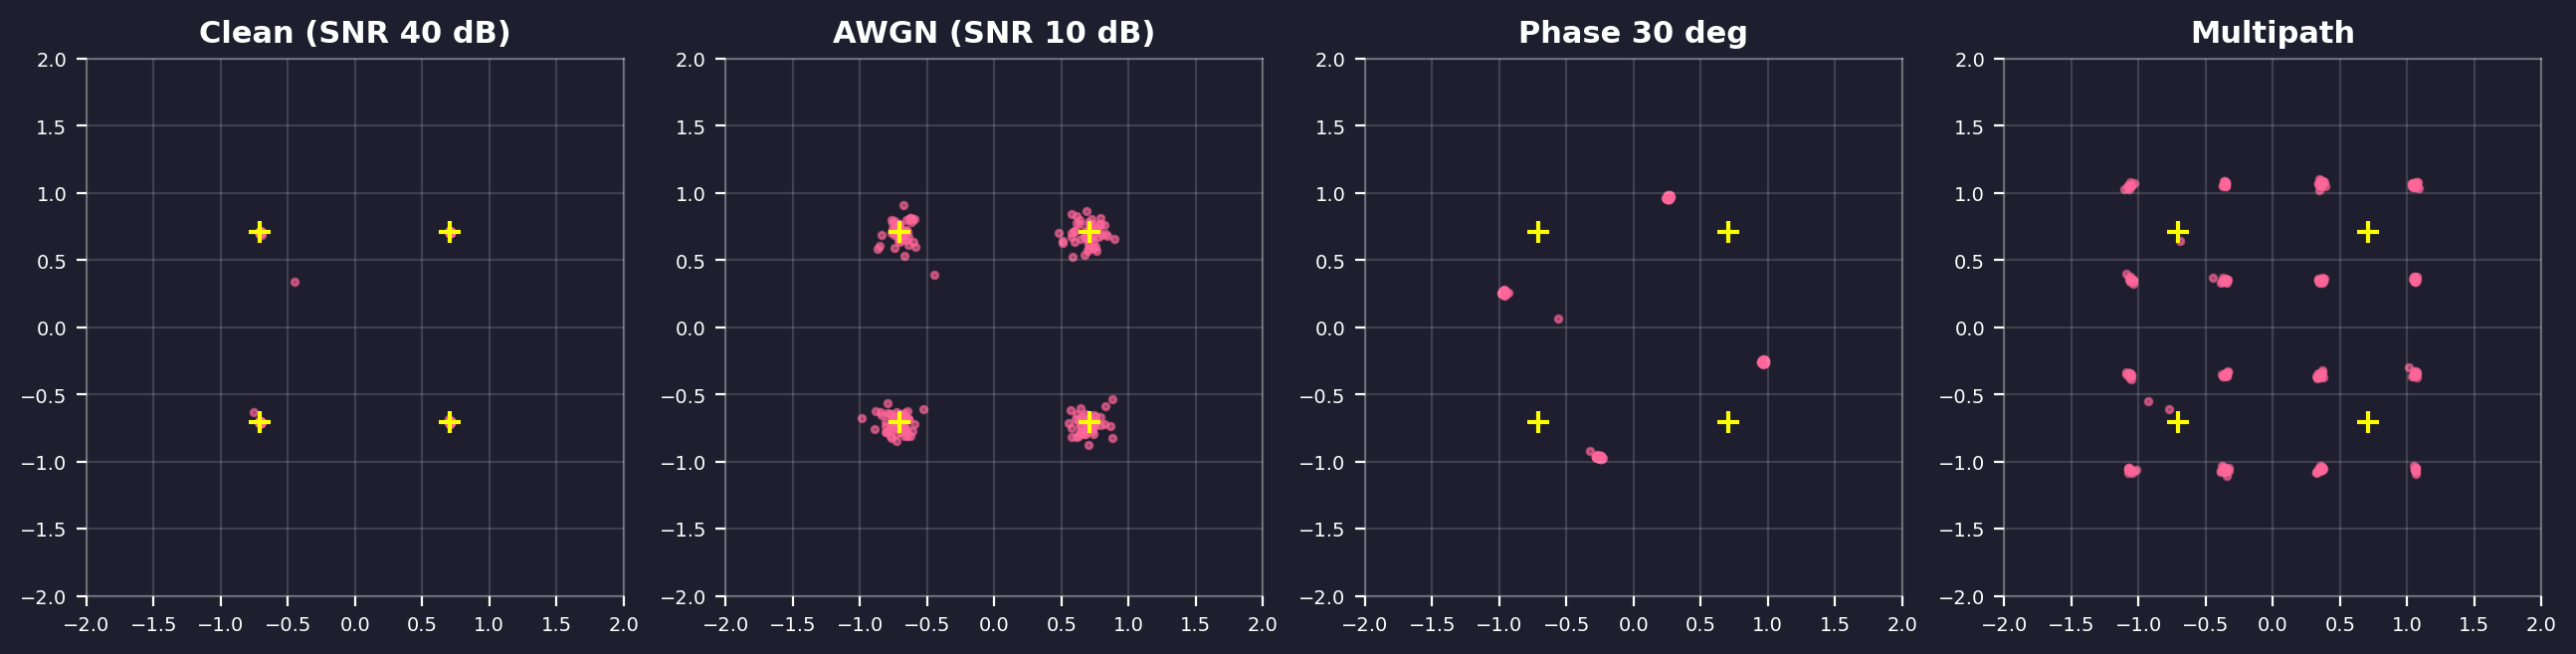
\includegraphics[width=0.92\textwidth]{figures/impairment_effects.png}
\end{center}
\vspace{-0.1cm}
\begin{center}
\small
\begin{tabular}{l l l}
\toprule
\textbf{Impairment} & \textbf{Model} & \textbf{Control Range} \\
\midrule
AWGN             & Complex Gaussian      & 0--40\,dB SNR \\
Phase offset     & $e^{j\phi}$ rotation  & $\pm 180^\circ$ \\
Frequency offset & Linear phase ramp     & $\pm 5000$\,Hz \\
Multipath        & 2-tap delay line      & 0--10 sym, gain 0--1 \\
Flat fading      & Rician envelope       & $K = -10$ to $40$\,dB \\
\bottomrule
\end{tabular}
\end{center}
\end{frame}

% ==================================================================
% SLIDE 7 -- Receiver Sync
% ==================================================================
\begin{frame}{Receiver Synchronization}
\begin{center}
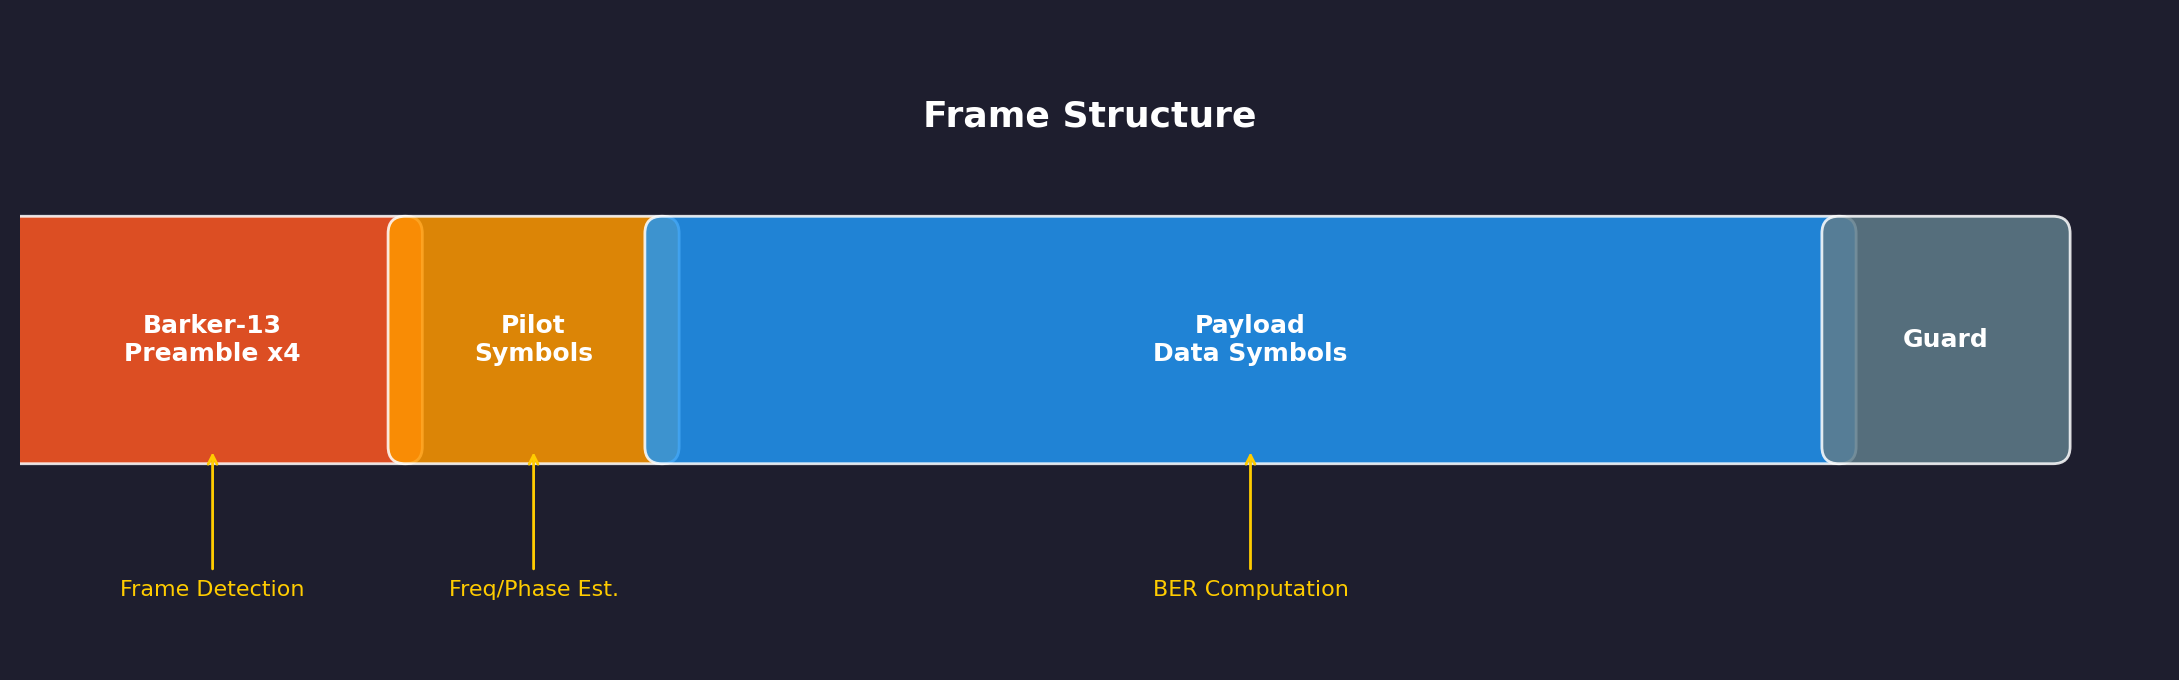
\includegraphics[width=0.85\textwidth]{figures/frame_structure.png}
\end{center}
\vspace{0.1cm}
\begin{columns}[T]
\begin{column}{0.48\textwidth}
\begin{enumerate}
    \item \textbf{Frame detection} -- cross-correlate with Barker-13 template
    \item \textbf{Freq offset est.} -- repeated-preamble phase difference
\end{enumerate}
\end{column}
\begin{column}{0.48\textwidth}
\begin{enumerate}\setcounter{enumi}{2}
    \item \textbf{Phase est.} -- pilot-aided from known preamble
    \item \textbf{Timing recovery} -- Gardner TED with first-order loop
\end{enumerate}
\end{column}
\end{columns}
\end{frame}

% ==================================================================
% SLIDE 8 -- Eye Diagram Deep Dive
% ==================================================================
\begin{frame}{Eye Diagram -- Reading Signal Health}
\begin{center}
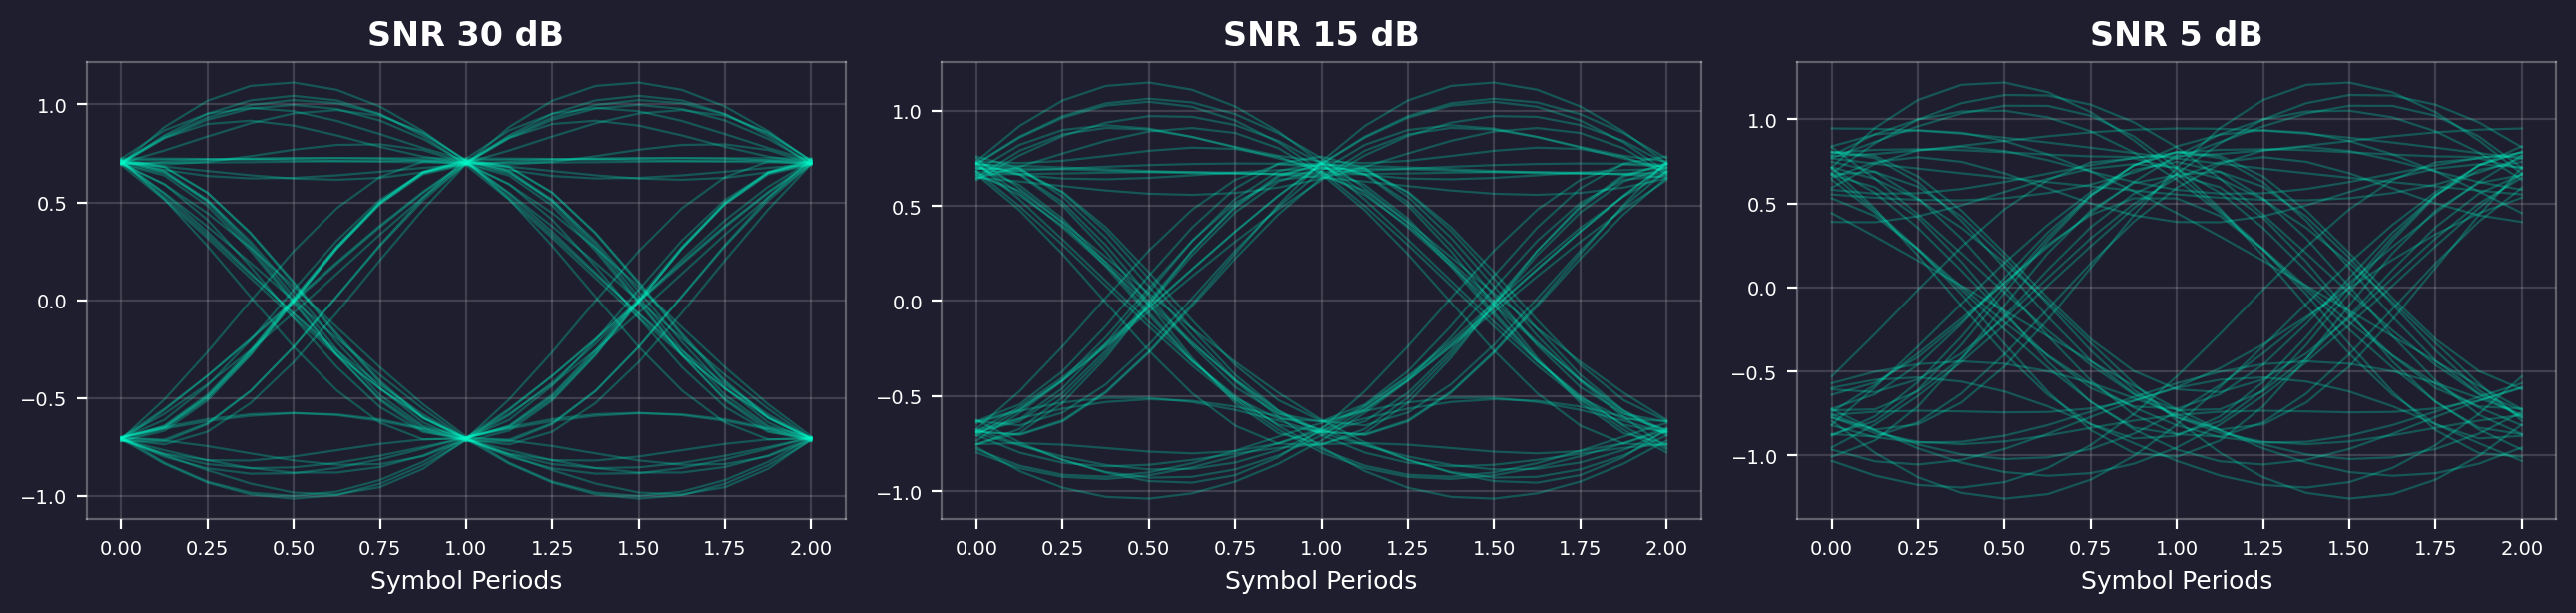
\includegraphics[width=0.88\textwidth]{figures/eye_diagrams.png}
\end{center}
\vspace{-0.1cm}
\begin{itemize}
    \item 50 overlaid symbol-period traces of the matched-filtered I channel
    \item \textbf{Wide-open eye} $\Rightarrow$ clean decisions \hfill
          \textbf{Closed eye} $\Rightarrow$ errors imminent
    \item Instantly shows ISI from multipath, jitter from timing error, or noise
\end{itemize}
\end{frame}

% ==================================================================
% SLIDE 9 -- Live GUI Walkthrough
% ==================================================================
\begin{frame}{Live Mode -- GUI Walkthrough}
\begin{center}
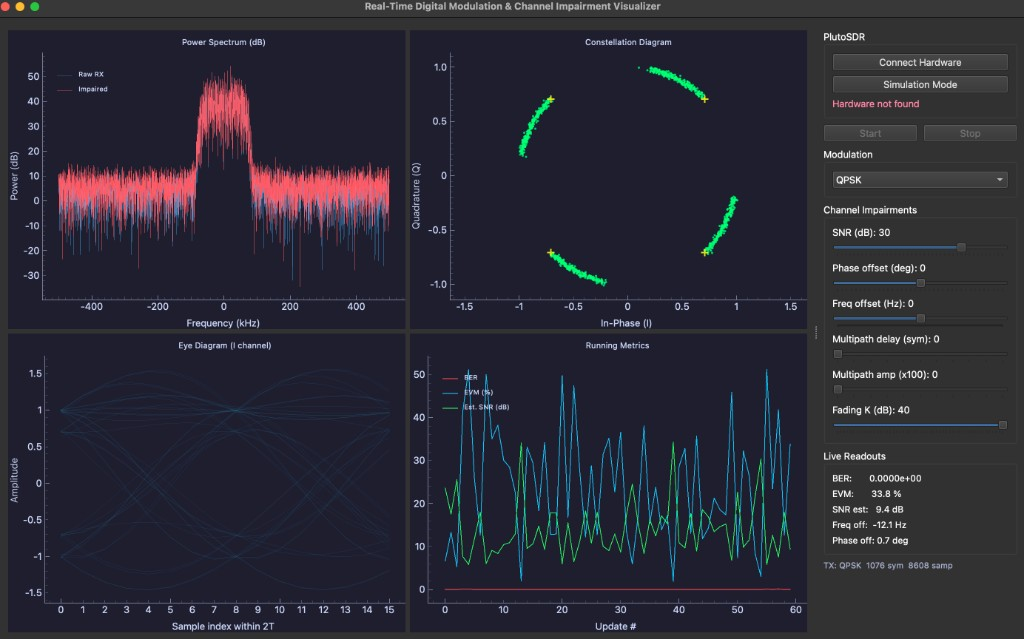
\includegraphics[width=0.82\textwidth]{figures/gui_live.png}
\end{center}
\vspace{-0.2cm}
\begin{columns}[T]
\begin{column}{0.24\textwidth}
\centering\small\textbf{Spectrum}\\FFT of IQ\\spectral shape
\end{column}
\begin{column}{0.24\textwidth}
\centering\small\textbf{Constellation}\\demod symbols\\ideal refs (yellow +)
\end{column}
\begin{column}{0.24\textwidth}
\centering\small\textbf{Eye Diagram}\\ISI indicator\\timing quality
\end{column}
\begin{column}{0.24\textwidth}
\centering\small\textbf{Metrics}\\rolling BER,\\EVM, SNR
\end{column}
\end{columns}
\vspace{0.15cm}
\centering\small + \textbf{Throughput \& Cumulative Bits} panel across the bottom row
\end{frame}

% ==================================================================
% SLIDE 10 -- BER Sweep Mode
% ==================================================================
\begin{frame}{BER Sweep Mode -- Theory Meets Measurement}
\begin{columns}[c]
\begin{column}{0.55\textwidth}
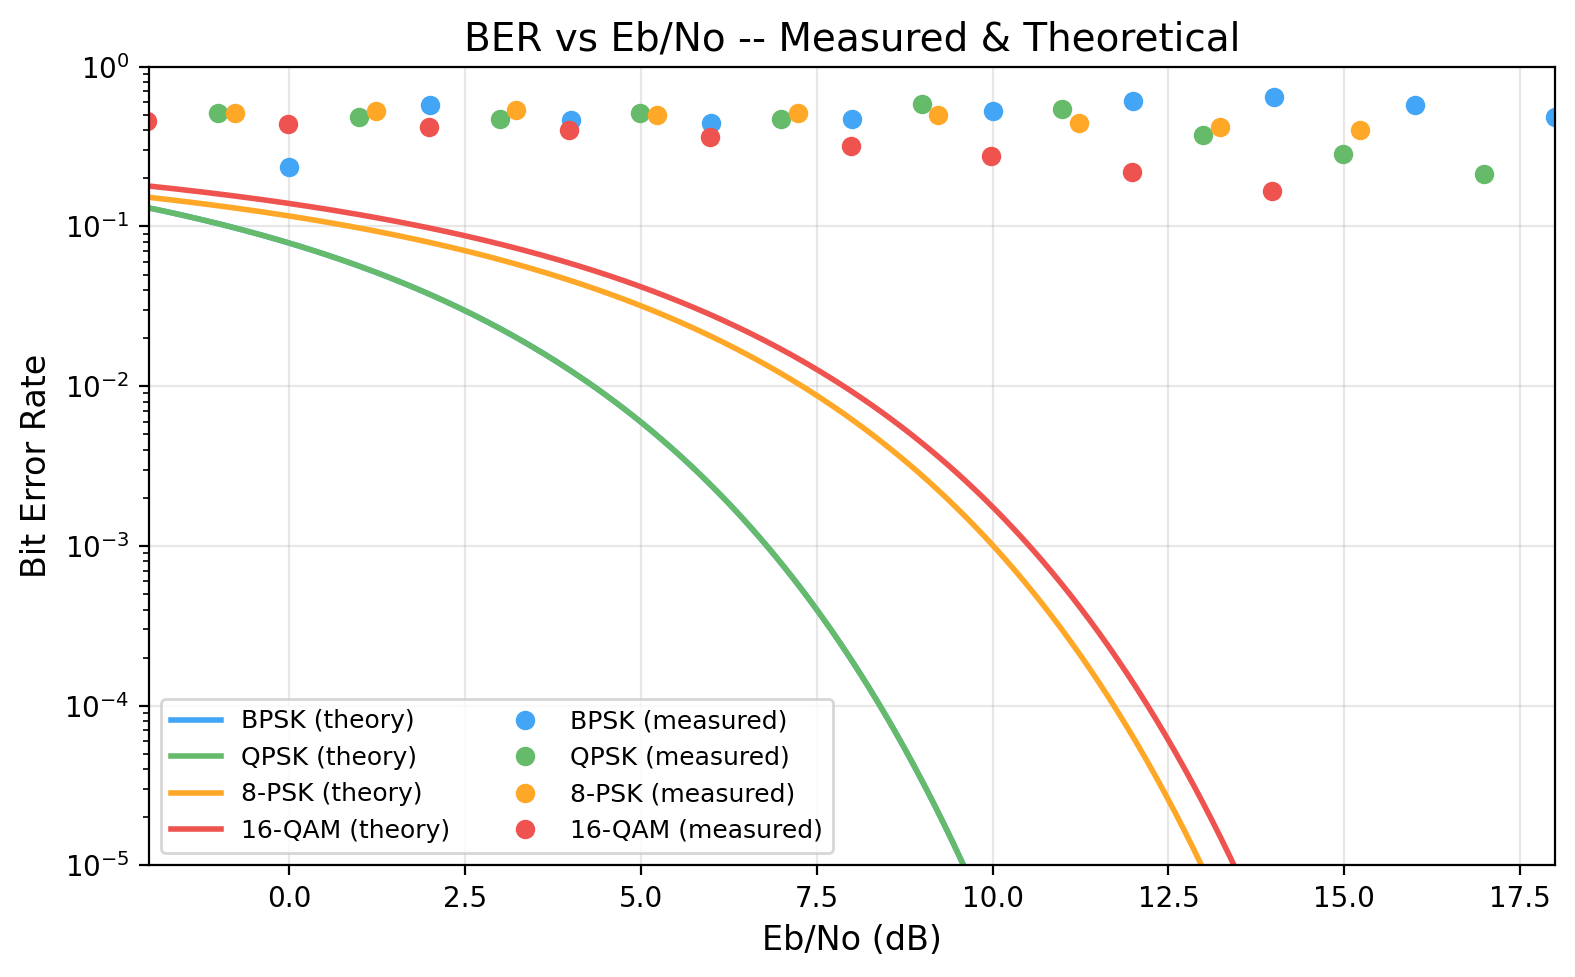
\includegraphics[width=\textwidth]{figures/ber_sweep.png}
\end{column}
\begin{column}{0.42\textwidth}
\begin{itemize}
    \item Automated: sweep SNR, measure BER for each scheme
    \item Circles = measured, dashed = theory:
    \begin{align*}
    \text{BPSK/QPSK:}\ & Q\!\bigl(\sqrt{2 E_b/N_0}\bigr) \\
    \text{16-QAM:}\ & \tfrac{3}{8}\,\text{erfc}\!\bigl(\sqrt{0.4\, E_b/N_0}\bigr)
    \end{align*}
    \item \alert{Validates} that our pipeline matches textbook curves
    \item Hardware loopback adds $\sim$0.5--1\,dB loss vs.\ simulation
\end{itemize}
\end{column}
\end{columns}
\end{frame}

% ==================================================================
% SLIDE 11 -- Throughput & Cumulative Bits
% ==================================================================
\begin{frame}{Throughput \& Cumulative Bits}
\begin{center}
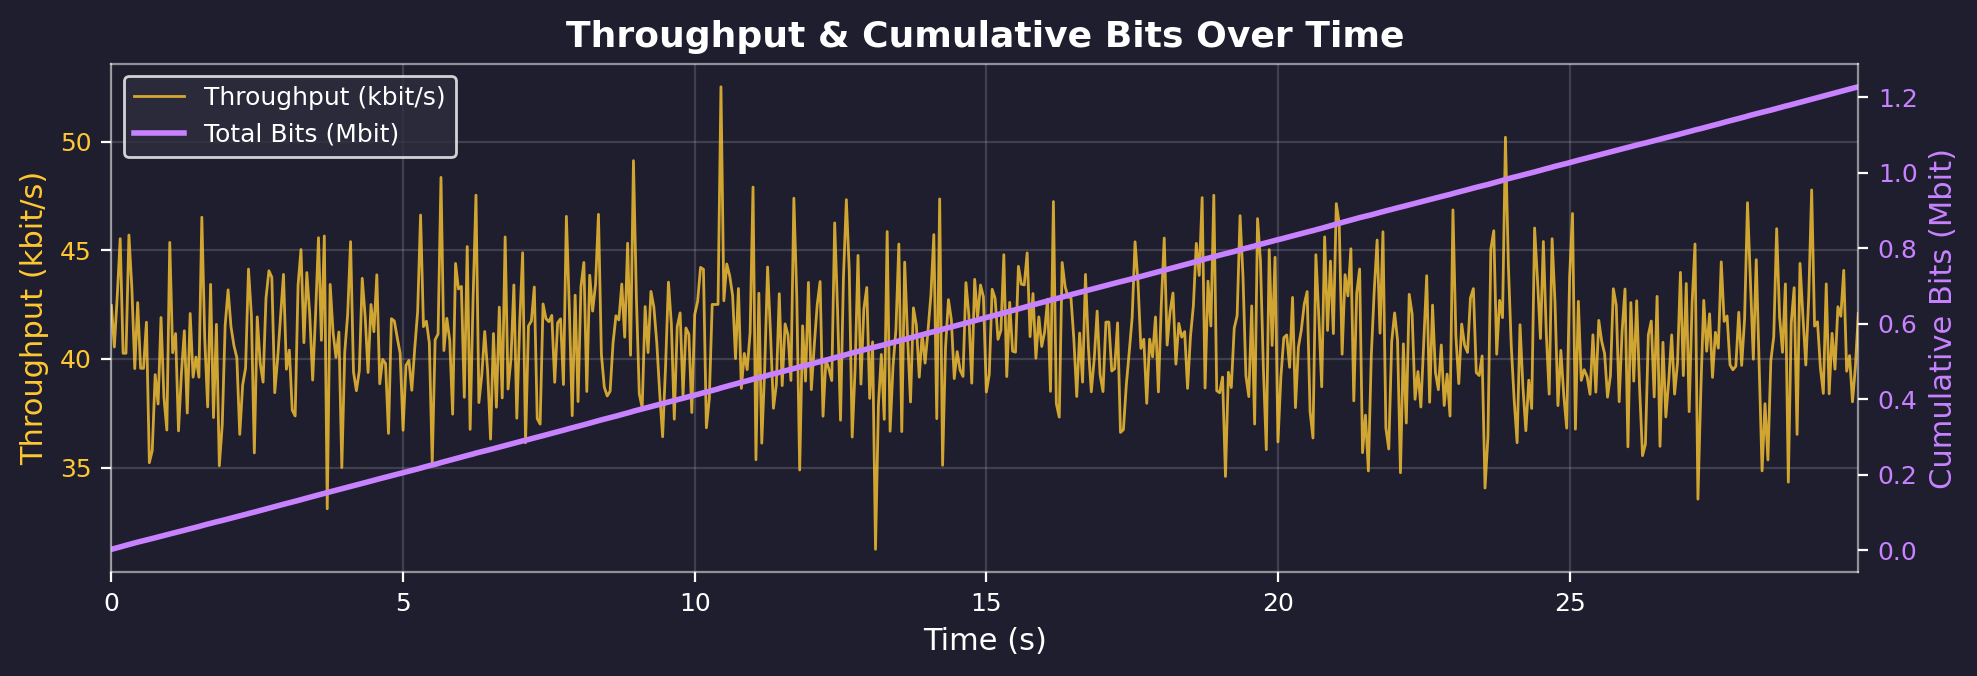
\includegraphics[width=0.88\textwidth]{figures/throughput_cumul.png}
\end{center}
\vspace{-0.2cm}
\begin{columns}[T]
\begin{column}{0.48\textwidth}
\begin{block}{Instantaneous Throughput}
\begin{itemize}
    \item QPSK at 20 FPS: $\sim$\alert{40 kbit/s} decoded payload
    \item 16-QAM doubles it: $\sim$80 kbit/s
    \item Varies with USB latency and sync lock
\end{itemize}
\end{block}
\end{column}
\begin{column}{0.48\textwidth}
\begin{block}{Cumulative Bits}
\begin{itemize}
    \item Tracks \textbf{every bit} decoded since ``Start''
    \item Linear ramp = steady link; plateau = sync loss
    \item $>$\,1\,Mbit within 30\,s of clean QPSK
\end{itemize}
\end{block}
\end{column}
\end{columns}
\end{frame}

% ==================================================================
% SLIDE 12 -- Software Design
% ==================================================================
\begin{frame}{Software Architecture}
\begin{center}
\small
\begin{tabular}{l l l}
\toprule
\textbf{Module} & \textbf{Role} & \textbf{Key Technique} \\
\midrule
\texttt{modulation.py}       & Constellation, mod/demod, RRC    & Gray-coded maps \\
\texttt{impairments.py}      & AWGN, phase, freq, multipath     & Chained transforms \\
\texttt{synchronization.py}  & Preamble, freq/phase/timing      & Gardner TED \\
\texttt{pluto\_interface.py} & PlutoSDR TX/RX                   & USB auto-detect \\
\texttt{dsp\_worker.py}      & QThread pipeline                 & Shared-data + mutex \\
\texttt{ber\_sweep.py}       & BER sweep engine                 & SNR loop + theory \\
\texttt{gui.py}              & PyQt6 + PyQtGraph                & 20 FPS timer poll \\
\bottomrule
\end{tabular}
\end{center}
\vspace{0.4cm}
\begin{block}{Key Design Choice}
DSP worker writes to shared memory $\to$ GUI timer reads at its own pace.\\
Result: \textbf{no signal-queue backlog}, consistent frame rate regardless of DSP speed.
\end{block}
\end{frame}

% ==================================================================
% SLIDE 12 -- Demo Scenarios
% ==================================================================
\begin{frame}{Demo Scenarios -- Try It Yourself}
\begin{columns}[T]
\begin{column}{0.48\textwidth}
\hlbox{green!50}{Noise Floor Exploration}
\begin{itemize}
    \item Start with all impairments off
    \item Slide SNR from 40\,dB $\to$ 0\,dB
    \item Watch: constellation spreads, eye closes, BER climbs
\end{itemize}
\vspace{0.3cm}
\hlbox{purple!60}{Multipath}
\begin{itemize}
    \item Delay = 3 symbols, gain = 0.5
    \item Eye diagram shows ISI directly
    \item Clusters blur and merge
\end{itemize}
\end{column}
\begin{column}{0.48\textwidth}
\hlbox{orange!60}{Phase \& Frequency Offset}
\begin{itemize}
    \item 45$^\circ$ phase: constellation rotates
    \item 2\,kHz freq offset: symbols spin (sync corrects it)
\end{itemize}
\vspace{0.3cm}
\hlbox{cyan!50}{Scheme Comparison}
\begin{itemize}
    \item Fix SNR at 15\,dB, switch BPSK $\to$ 16-QAM
    \item More bits/symbol = less noise margin
    \item BER sweep quantifies the trade-off
\end{itemize}
\end{column}
\end{columns}
\end{frame}

% ==================================================================
% SLIDE 13 -- Results
% ==================================================================
\begin{frame}{Results \& Observations}
\begin{columns}[T]
\begin{column}{0.50\textwidth}
\begin{block}{Quantitative}
\begin{itemize}
    \item Measured BER curves match theory within $<$\,1\,dB for all four schemes
    \item Hardware loopback adds $\sim$0.5--1\,dB loss (I/Q imbalance, DC offset, quantization)
    \item Gardner TED locks timing within 2--3 symbol periods
\end{itemize}
\end{block}
\end{column}
\begin{column}{0.46\textwidth}
\begin{block}{Performance}
\begin{itemize}
    \item Simulation mode: $\sim$20 FPS, 6\,ms DSP/frame
    \item Hardware mode: $\sim$15 FPS (USB latency)
    \item Sustained $\sim$40\,kbit/s (QPSK) to $\sim$80\,kbit/s (16-QAM) decoded throughput
    \item $>$\,1\,Mbit cumulative within 30\,s
\end{itemize}
\end{block}
\end{column}
\end{columns}
\end{frame}

% ==================================================================
% SLIDE 14 -- What I Learned
% ==================================================================
\begin{frame}{Lessons Learned}
\begin{enumerate}
    \item \textbf{Synchronization is the hard part} -- modulation is textbook, but preamble detection + timing recovery required iterative tuning
    \item \textbf{Decouple DSP from GUI} -- direct signal emissions caused Qt event-queue backlog; shared memory + timer polling fixed it
    \item \textbf{Hardware surprises} -- real PlutoSDR has DC offset, I/Q imbalance, and USB latency that pure math ignores
    \item \textbf{Visualization builds intuition} -- watching the constellation rotate under frequency offset taught me more than any derivation
\end{enumerate}
\end{frame}

% ==================================================================
% SLIDE 15 -- Conclusion
% ==================================================================
\begin{frame}{Conclusion}
\begin{center}
\begin{minipage}{0.85\textwidth}
\large
Built a \alert{complete real-time digital communications visualizer} with:
\vspace{0.3cm}
\begin{itemize}
    \item[\checkmark] 4 modulation schemes (BPSK, QPSK, 8-PSK, 16-QAM)
    \item[\checkmark] 6 controllable channel impairments with instant visual feedback
    \item[\checkmark] Full receiver synchronization chain
    \item[\checkmark] Live throughput \& cumulative bits tracking
    \item[\checkmark] Two modes: interactive live exploration \& automated BER sweep
    \item[\checkmark] Hardware or simulation -- works everywhere
\end{itemize}
\vspace{0.5cm}
All open-source Python -- $\sim$1200 lines across 7 modules.
\end{minipage}
\end{center}
\vfill
\begin{center}
\Large\textbf{\color{yellow!80}Thank You -- Questions?}
\end{center}
\end{frame}

\end{document}
